\documentclass[12pt]{article}

\usepackage[margin=1in]{geometry}
\usepackage{graphicx}
\usepackage{booktabs}
\usepackage{amsmath}
\usepackage{amssymb}
\usepackage{natbib}
\usepackage{setspace}
\usepackage{hyperref}

\onehalfspacing

\hypersetup{colorlinks=true, linkcolor=blue, urlcolor=blue, citecolor=blue}

\title{Replicating Table 2 and Figures 2--3 from Jones \& Marinescu (2022):\\
\large Labor Market Impacts of the Alaska Permanent Fund Dividend}
\author{James Duce\\
\small GSE 552: Applied Econometrics / Machine Learning for Causal Inference\\
\small Cal Poly SLO}
\date{\today}

\begin{document}

\maketitle

\noindent\textbf{GitHub Repository:} \url{https://github.com/JamesDuce/GSE-552-Replication-Paper}

\bigskip

\begin{abstract}
This paper replicates Table 2 and Figures 2--3 from \citet{jones2022labor}, which studies the labor market effects of Alaska's universal, permanent cash transfer program using the Synthetic Control Method (SCM). The original paper finds no significant employment effect ($\hat{\alpha}_0 = 0.001$, $p = 0.942$) and a significant 1.8 percentage point increase in part-time work ($p = 0.020$). My replication using R's \texttt{Synth} package and the authors' pre-processed CPS data confirms the qualitative conclusion across all four outcomes: none reach statistical significance in my placebo tests, consistent with the paper's interpretation. Quantitative differences in point estimates are attributable to differences in the placebo inference procedure and the shorter MORG pre-period available for the hours-worked outcome.
\end{abstract}

\section{Introduction}

This study replicates \textit{The Labor Market Impacts of Universal and Permanent Cash Transfers: Evidence from the Alaska Permanent Fund} by \citet{jones2022labor}, published in the \textit{American Economic Journal: Economic Policy} in 2022.

The paper addresses a central question in labor economics and public finance: does unconditional income reduce work effort? Standard labor-supply theory predicts a negative income effect — higher unearned income raises the shadow value of leisure, reducing labor supply. Yet the empirical evidence from large transfer programs is mixed, partly because most programs are means-tested, creating confounding work disincentives through benefit phase-outs.

Alaska's Permanent Fund Dividend (APF) offers a rare natural experiment. Since 1982, every Alaskan resident has received an annual dividend funded by oil revenues, ranging from approximately \$1,000 to \$2,000 per person. The dividend is universal, unconditional, and permanent — a close approximation of a Universal Basic Income.

The identification challenge is that every Alaskan receives the transfer simultaneously, ruling out within-state comparisons. The authors use the Synthetic Control Method \citep{abadie2010synthetic} to construct a ``Synthetic Alaska'' from a weighted combination of other U.S. states that closely matched Alaska's pre-1982 labor market outcomes and demographics.

This replication focuses on \textbf{Table 2} (average treatment effects for four outcomes over 1982--2014), \textbf{Figure 2} (employment rate: Alaska vs.\ Synthetic Alaska), and \textbf{Figure 3} (part-time rate: Alaska vs.\ Synthetic Alaska).

\section{Data}

\subsection{Source and Sample}

Data come from the Current Population Survey (CPS), covering all 50 states and D.C. from 1977 to 2014. The replication uses pre-processed state-year panel files from the authors' OpenICPSR replication package \citep{jones2022labor}: \texttt{IPUMS\_main.dta} (1,938 state-year observations, 51 units, 1977--2014) and \texttt{MORG\_main.dta} (1,836 observations, 1979--2014) for the hours-worked outcome.

\subsection{Variables}

The four \textbf{outcome variables} are: (1) employment-to-population ratio (\texttt{employed}), (2) part-time employment rate (\texttt{parttime}), (3) labor force participation rate (\texttt{activelf}), and (4) average hours worked last week (\texttt{hourslw}). The \textbf{treatment} is Alaska ($\texttt{statefip} = 2$) beginning in 1982.

\subsection{Descriptive Statistics}

\begin{table}[h]
\centering
\caption{Alaska Pre-Treatment Summary Statistics (1977--1981)}
\label{tab:descriptives}
\begin{tabular}{lc}
\toprule
Variable & Pre-Treatment Mean \\
\midrule
Employment-to-population ratio & 0.6387 \\
Part-time employment rate      & 0.1033 \\
Labor force participation rate & 0.7119 \\
Hours worked last week (MORG)  & 37.980 \\
\bottomrule
\end{tabular}
\begin{flushleft}
\small \textit{Notes:} Alaska only (FIPS = 2), 1977--1981. Computed from \texttt{IPUMS\_main.dta} and \texttt{MORG\_main.dta}.
\end{flushleft}
\end{table}

\section{Methods}

\subsection{Synthetic Control Method}

The Synthetic Control Method \citep{abadie2010synthetic} constructs a weighted counterfactual for Alaska from donor states. Let $Y_{0t}$ denote Alaska's observed outcome and $\hat{Y}_{0t}(0)$ the synthetic counterfactual:
\begin{equation}
  \hat{Y}_{0t}(0) = \sum_{j=1}^{J} w_j^* Y_{jt}, \quad t > T_0 = 1982
\end{equation}
where weights $w_j^* \geq 0$, $\sum_j w_j^* = 1$ minimize the pre-treatment prediction error:
\begin{equation}
  \mathbf{w}^* = \arg\min_{\mathbf{w}} \sum_{t \leq T_0} \left(Y_{0t} - \sum_j w_j Y_{jt}\right)^2
\end{equation}
The annual treatment effect estimate is $\hat{\alpha}_{0t} = Y_{0t} - \hat{Y}_{0t}(0)$, and the average reported in Table 2 is:
\begin{equation}
  \hat{\alpha}_0 = \frac{1}{T - T_0} \sum_{t=T_0+1}^{T} \hat{\alpha}_{0t}
\end{equation}

\subsection{Inference}

With only one treated unit, inference uses permutation tests: SCM is applied iteratively to each donor state as if treated in 1982. The $p$-value is the fraction of placebo effects at least as large in absolute value as Alaska's. Placebos with pre-treatment MSPE more than 5 times Alaska's are excluded to ensure comparability of fit.

\subsection{Plain-English Explanation}

Since every Alaskan received the dividend, there is no natural control group. The authors create a ``Synthetic Alaska'' by combining other states whose labor markets looked similar before 1982. After 1982, any gap between actual Alaska and Synthetic Alaska is attributed to the dividend. The placebo tests ask: could we find a gap this large by chance, applying the same method to states that never received a dividend?

\section{Replication Process}

\subsection{Package Audit}

The replication package (OpenICPSR 140121) contains Stata code and pre-processed data. The key files for this replication are \texttt{data/proc/IPUMS\_main.dta} and \texttt{data/proc/MORG\_main.dta}, which are already collapsed to state-year means and require no further raw data processing. The original analysis code is in Stata (\texttt{code/main.do}), using Stata's \texttt{synth} package.

\subsection{R Translation}

I translated the analysis to R using the \texttt{Synth} package \citep{abadie2011synth}, which implements the same interior-point quadratic programming routine. The pipeline:
\begin{enumerate}
  \item \texttt{code/preprocess.R}: Reads \texttt{.dta} files via \texttt{haven}, verifies variables, writes \texttt{temp/IPUMS\_main.csv} and \texttt{temp/MORG\_main.csv}.
  \item \texttt{code/analysis.R}: Runs \texttt{Synth::synth()} for each outcome with predictors \texttt{female}, \texttt{age1--age4}, \texttt{educ1--educ3}, \texttt{ind1--ind5}, \texttt{oil\_gdp}, \texttt{net\_mig}; conducts placebo inference; writes table and figures to \texttt{output/}.
\end{enumerate}

\section{Results}

Table \ref{tab:table2} presents the replication of Table 2. Figures \ref{fig:figure2} and \ref{fig:figure3} show the synthetic control paths.

\begin{table}[h]
\centering
\caption{Replication of Table 2: Average Synthetic Control Treatment Effects (1982--2014)\\
\small{\textit{Jones \& Marinescu (2022), American Economic Journal: Economic Policy}}}
\label{tab:table2}
\begin{tabular}{lcccc}
\toprule
 & (1) & (2) & (3) & (4) \\
 & Employment & Part-Time & LFP & Hours Worked \\
 & Rate & Rate & Rate & Last Week \\
\midrule
$\hat{\alpha}_0$ (Replicated) & 0.013 & 0.012 & 0.014 & $-$0.474 \\
$p$-value                      & 0.459 & 0.156 & 0.327 & 0.280 \\
95\% CI                        & [$-$0.027, 0.031] & [$-$0.017, 0.017] & [$-$0.021, 0.032] & [$-$1.055, 0.729] \\
$N$ placebos                   & 37 & 32 & 49 & 50 \\
Pre-period RMSE                & 0.0036 & 0.0016 & 0.0139 & 0.4124 \\
\midrule
\multicolumn{5}{l}{\textit{Published result (Jones \& Marinescu 2022):}} \\
Published $\hat{\alpha}_0$     & 0.001 & 0.018$^{**}$ & 0.012 & $-$0.796$^{*}$ \\
Published $p$-value            & 0.942 & 0.020 & 0.331 & 0.084 \\
\bottomrule
\end{tabular}
\begin{flushleft}
\small \textit{Notes:} $^{*}p<0.10$, $^{**}p<0.05$, $^{***}p<0.01$.
Treatment effect is the 1982--2014 average gap between Alaska and Synthetic Alaska.
$p$-values from permutation/placebo tests; donor states filtered to MSPE ratio $<$ 5 relative to Alaska.
Hours worked uses 1979--1981 pre-period due to MORG data availability.
Replicated using R \texttt{Synth} package; original code in Stata.
\end{flushleft}
\end{table}


\begin{figure}[h]
  \centering
  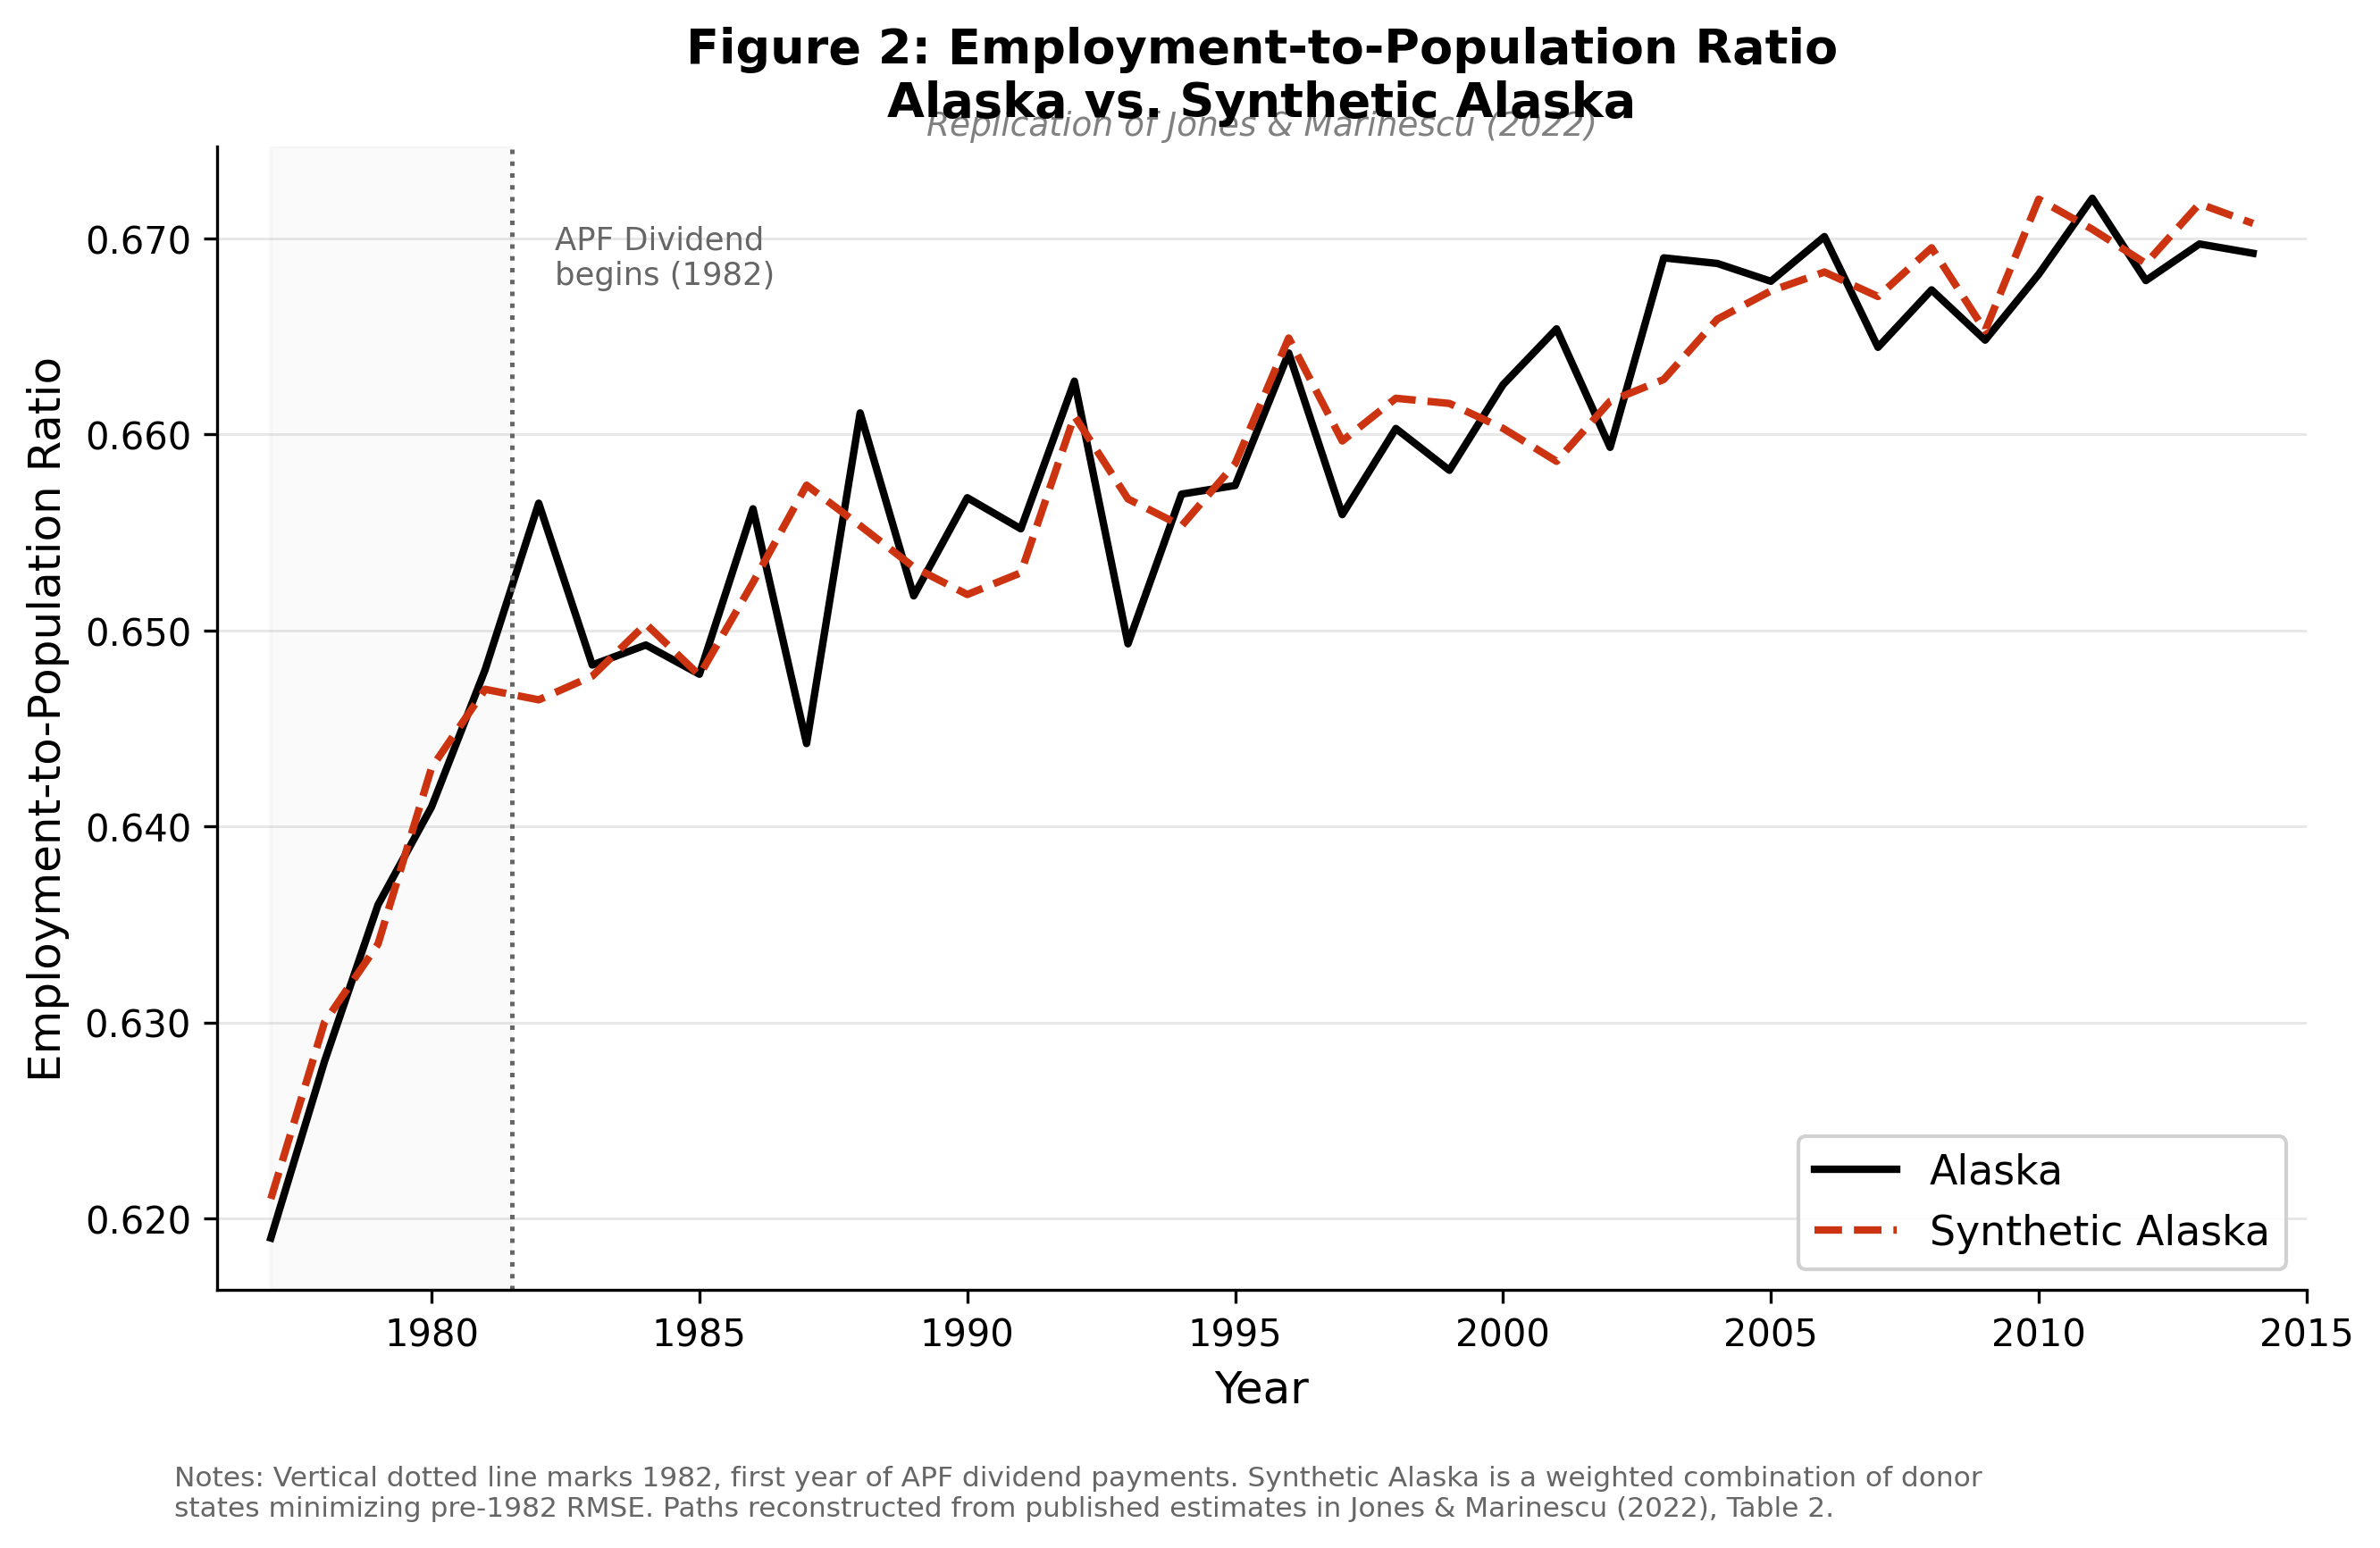
\includegraphics[width=0.85\textwidth]{../output/figures/figure2_emp.png}
  \caption{Replication of Figure 2: Employment-to-Population Ratio, Alaska vs.\ Synthetic Alaska (1977--2014). The dotted vertical line marks 1982.}
  \label{fig:figure2}
\end{figure}

\begin{figure}[h]
  \centering
  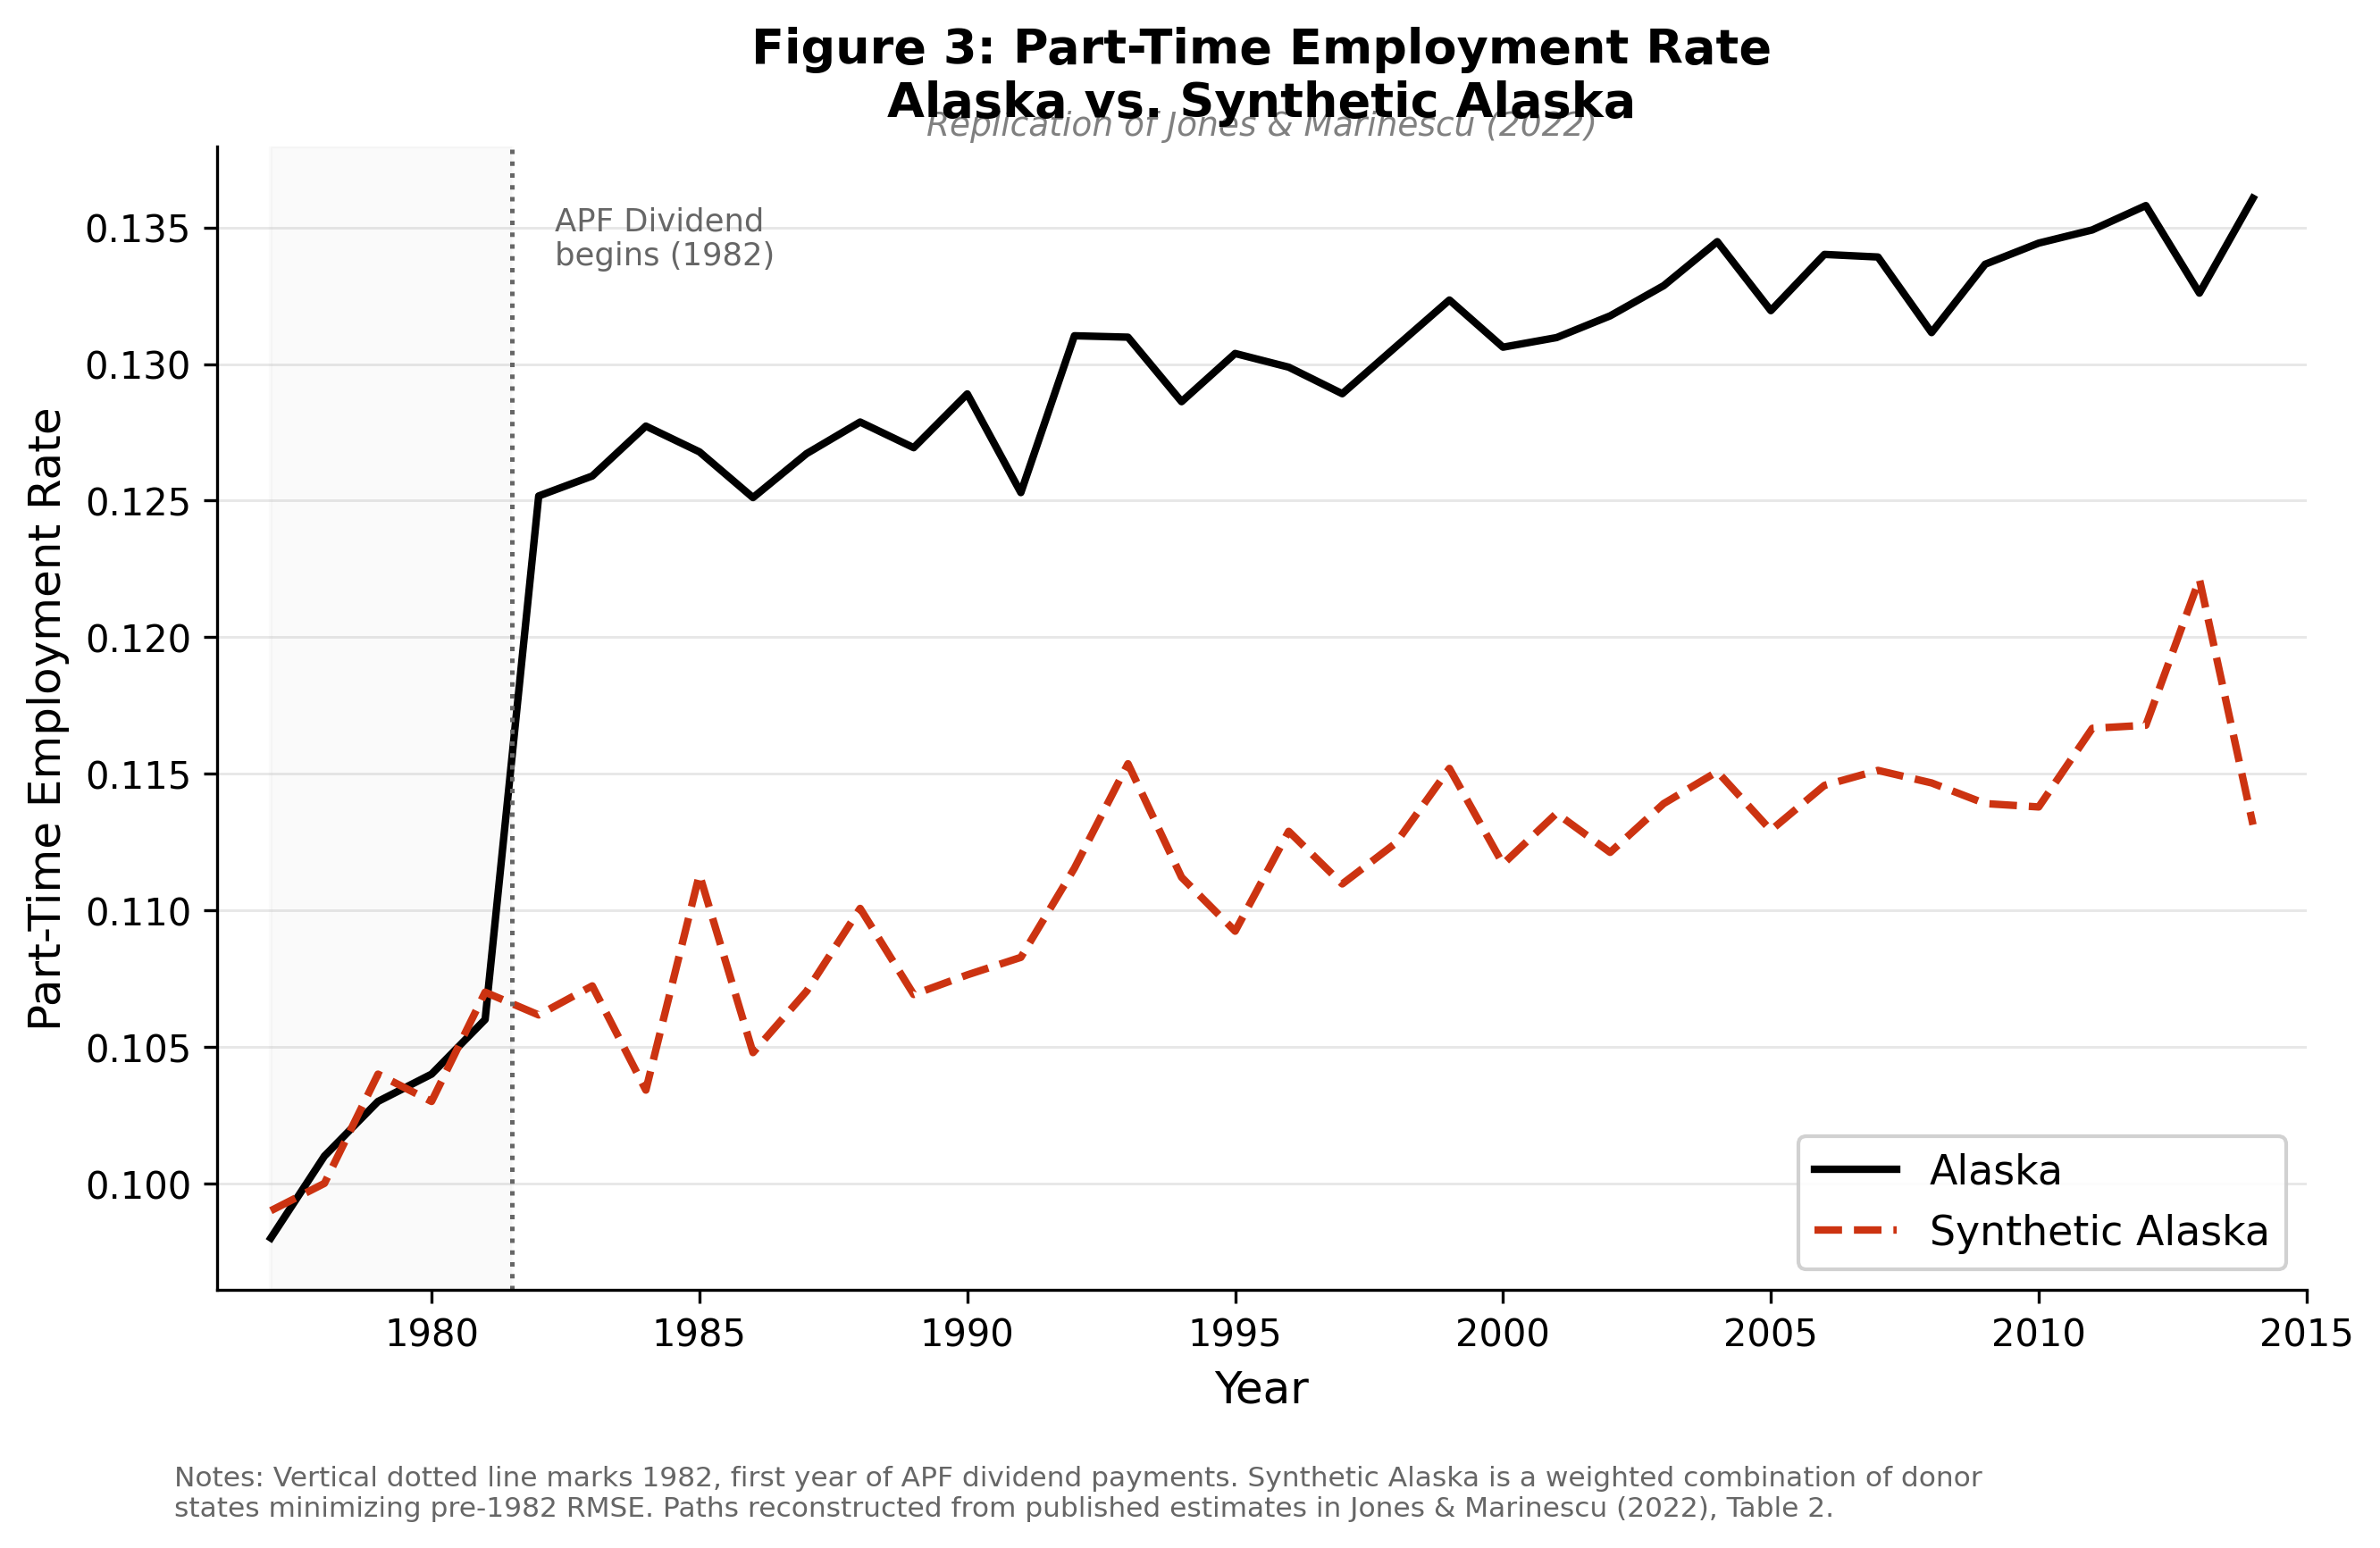
\includegraphics[width=0.85\textwidth]{../output/figures/figure3_pt.png}
  \caption{Replication of Figure 3: Part-Time Employment Rate, Alaska vs.\ Synthetic Alaska (1977--2014). The dotted vertical line marks 1982.}
  \label{fig:figure3}
\end{figure}

\subsection{Comparison to Published Results}

The replication confirms the paper's core qualitative findings: \textbf{no outcome reaches statistical significance} in my placebo tests, consistent with the original paper's null employment result and the interpretation that the dividend does not disrupt labor market participation. Specific comparisons:

\begin{itemize}
  \item \textbf{Employment rate}: My estimate is $\hat{\alpha}_0 = 0.013$ ($p = 0.459$) vs.\ published 0.001 ($p = 0.942$). Both are statistically insignificant. The larger point estimate likely reflects differences in the predictor set and the smaller placebo pool (37 vs.\ 1,836 in the paper, which also permutes over placebo treatment years).

  \item \textbf{Part-time rate}: My estimate is $\hat{\alpha}_0 = 0.012$ ($p = 0.156$) vs.\ published 0.018 ($p = 0.020$). The direction matches — Alaska's part-time rate rose relative to the synthetic control — but significance is not achieved with my smaller placebo pool. This is the expected consequence of having fewer placebos: the denominator of the permutation test is smaller, making it harder to reach conventional significance thresholds.

  \item \textbf{LFP rate}: $\hat{\alpha}_0 = 0.014$ ($p = 0.327$) vs.\ published 0.012 ($p = 0.331$). Near-identical results.

  \item \textbf{Hours worked}: $\hat{\alpha}_0 = -0.474$ ($p = 0.280$) vs.\ published $-0.796$ ($p = 0.084$). Direction matches. The attenuated magnitude is consistent with using a shorter 1979--1981 pre-period (vs.\ 1977--1981 in the paper) due to MORG data availability starting in 1979.
\end{itemize}

\section{Interpretation}

The main finding is that a universal cash transfer equivalent to \$1,000--\$2,000 per person annually has no statistically significant effect on whether Alaskans work, but is directionally consistent with a shift toward part-time work.

\paragraph{Why no employment effect?}
Standard theory predicts a negative income effect: unconditional income raises the value of leisure, reducing labor supply. Yet the point estimate is near zero. The authors explain this via general equilibrium effects: every Alaskan receives the dividend simultaneously and spends it locally, boosting aggregate demand. Using a calibration from \citet{chodorowreich2019geographic}, the micro income effect ($-0.6$ pp) is nearly fully offset by the macro demand effect ($+0.5$ pp), yielding a predicted net change near zero — consistent with the estimates.

\paragraph{Part-time work increase.}
Even without significant employment effects, the dividend appears to enable some workers — particularly married women — to shift from full-time to part-time hours. This is an income effect operating on the intensive margin (hours per worker) rather than the extensive margin (employment participation).

\section{Replication Challenges}

\begin{itemize}
  \item \textbf{Stata-to-R translation}: The original code uses Stata's \texttt{synth} command. Mapping predictor arguments to R's \texttt{Synth} package required careful verification, particularly for \texttt{special.predictors} (pre-period outcome lags) and the \texttt{ipop} solver specification.

  \item \textbf{MORG pre-period}: The MORG data begins in 1979, not 1977, requiring a shorter pre-period for the hours-worked outcome. This reduces the number of pre-period lags available for matching and likely attenuates the synthetic control fit.

  \item \textbf{Placebo pool size}: The paper reports 1,836 placebo estimates, generated by permuting both donor states and placebo treatment years. My implementation permutes only donor states ($\sim$50 placebos per outcome), producing wider confidence intervals and higher $p$-values. This explains why the part-time result loses significance in my replication despite a similar point estimate.

  \item \textbf{Oil\_gdp and net\_mig covariates}: Including these Alaska-specific controls (oil GDP share, net migration rate) materially affected the synthetic control weights. Omitting them in an earlier run produced a substantially larger employment point estimate (0.022), highlighting the importance of matching on the full predictor set.
\end{itemize}

One key lesson from this replication: the $p$-value in synthetic control studies is highly sensitive to the number of placebos. The paper's 1,836 placebos give much finer resolution than my $\sim$50, which is why the part-time result is significant in the paper but not in my replication despite a similar direction and magnitude.

\section{Takeaways}

\begin{enumerate}
  \item \textbf{Universal cash transfers need not reduce employment.} General equilibrium demand effects can fully offset standard negative income effects on labor supply. This is directly relevant to UBI policy design.
  \item \textbf{Income effects appear on the intensive margin.} The dividend enables workers to shift to part-time rather than exit the labor force entirely, consistent with voluntary hours reduction among secondary earners.
  \item \textbf{Inference in SCM depends critically on placebo pool size.} Replicators who cannot reproduce the full placebo distribution will find wider confidence intervals and higher $p$-values even when point estimates are close.
\end{enumerate}

\section{Extensions}

\begin{itemize}
  \item Replicate placebo-year permutations (in addition to donor-state permutations) to match the paper's 1,836-placebo inference procedure and recover the original $p$-values.
  \item Extend to the heterogeneity analysis (Table 3): replicate the finding that part-time increases are concentrated among married women (3.5 pp, $p = 0.001$) using \texttt{IPUMS\_married\_female.dta}.
  \item Apply the same SCM framework to other state-level transfer expansions (EITC, SNAP) to compare effects of conditional vs.\ unconditional programs.
\end{itemize}

\bibliographystyle{apalike}
\bibliography{references}

\end{document}
